\newpage

\subsection{QuizziPedia::Front-End::Views}
\subsubsection{Informazioni generali}
\label{QuizziPedia::Front-End}
\begin{figure}
	\centering
	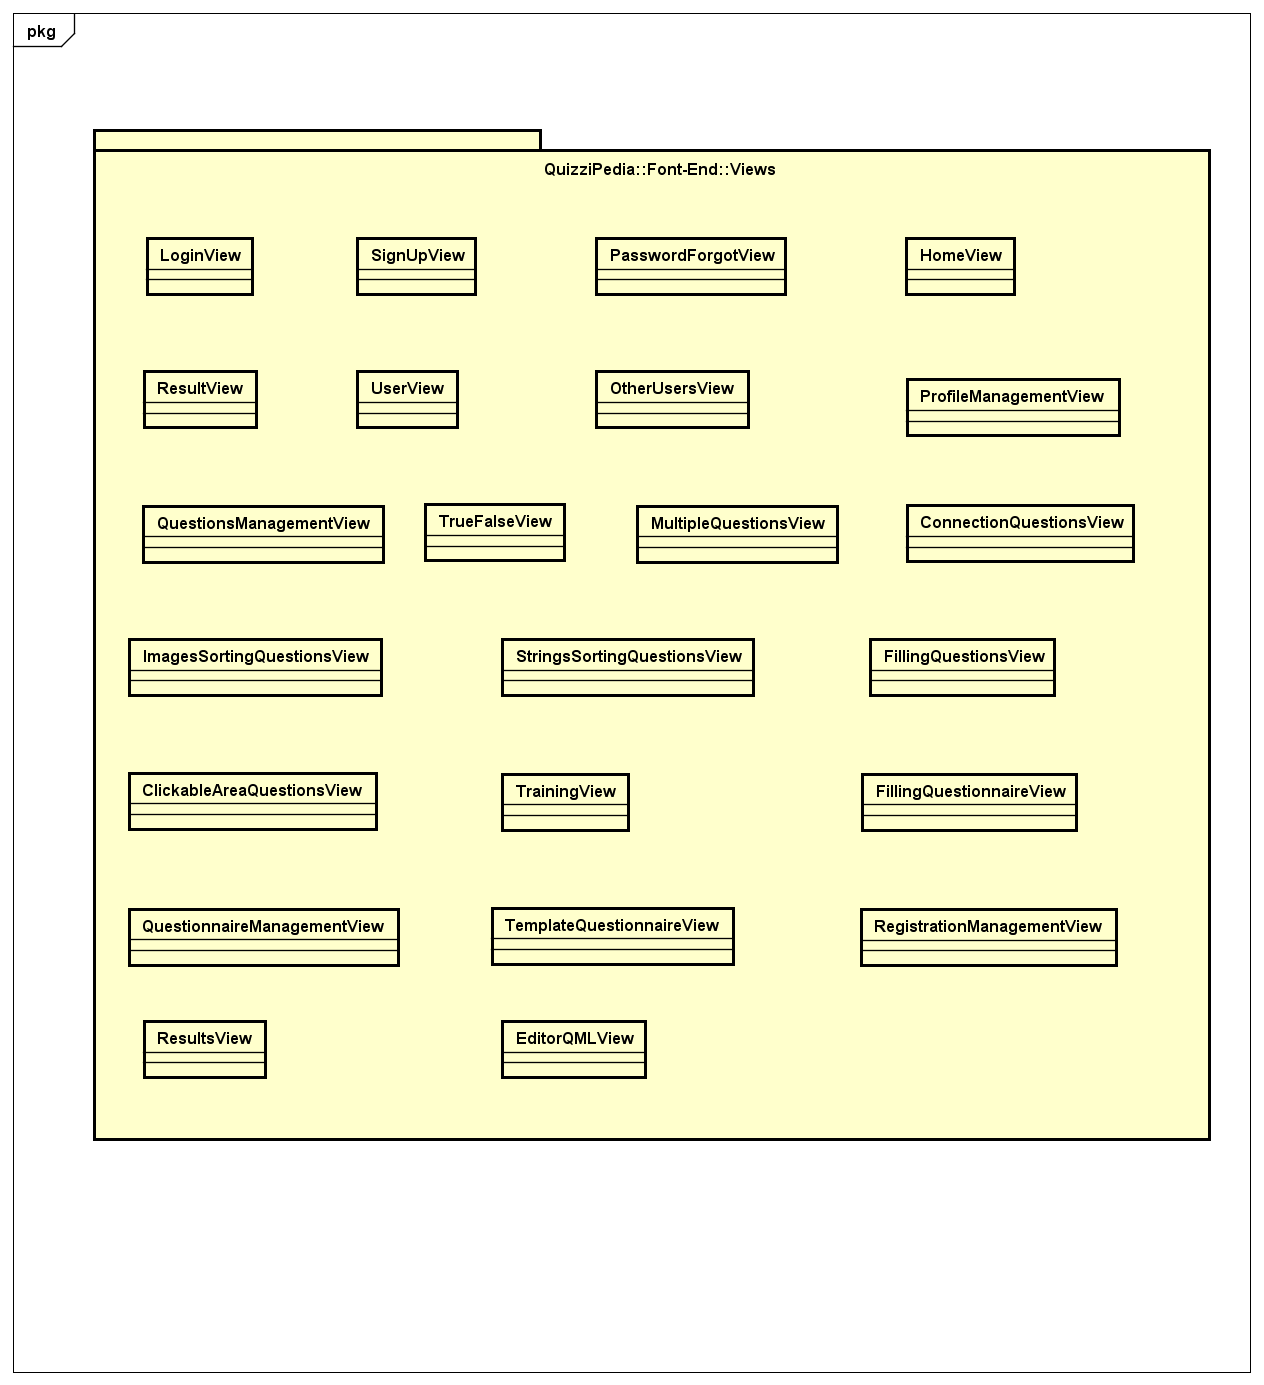
\includegraphics[scale=0.45]{UML/Package/QuizziPedia_Front-End_View.png}
	\caption{QuizziPedia::Front-End::Views}
\end{figure}
\begin{itemize}
	\item \textbf{Descrizione}: package contenente le views front-end dell'applicazione.
	\item \textbf{Padre}: \texttt{Front-End}
	\item \textbf{Interazione con altri componenti}:
	\begin{itemize}
		\item \texttt{Controllers}: package contenente i controllers front-end dell'applicazione.
		\item \texttt{Directives}: package contenente le directives front-end dell'applicazione.
		\item \texttt{Models}: package contenente le classi che definiscono la business logic dell'applicazione.
		\item \texttt{Templates}: package contenente i templates front-end dell'applicazione.
	\end{itemize}
\end{itemize}
\subsubsection{Classi}

\paragraph{QuizziPedia::Front-End::Views::Index}
\begin{itemize}
	\item \textbf{Descrizione}:  view generale dell'applicazione;
	\item \textbf{Utilizzo}: contiene gli elementi che saranno presenti in ogni pagina dell'applicazione;
	\item \textbf{Relazioni con altre classi}:
	\begin{itemize}
		\item \textit{IN} \texttt{MenuBarDirective}: rappresenta il menù, presente in ogni pagina dell'applicazione, generato in base agli oggetti passati nello \$scope isolato. Fornisce un pulsante per ogni oggetto ricevuto come parametro, ogni pulsante viene rappresentato con un’icona e con un testo. Al click di un pulsante viene invocata la funzione ad esso associata;
		\item \textit{IN} \texttt{ErrorsDirective}: directive che mostra l'eventuale errore dopo un'azione;
		\item \textit{IN} \texttt{FooterDirective}: directive che mostra il footer dell'applicazione che sarà presente in ogni pagina;
	\end{itemize}
	\item \textbf{Attributi}
\end{itemize}

\paragraph{QuizziPedia::Front-End::Views::LoginView}
\begin{itemize}
	\item \textbf{Descrizione}: view contenente le form necessarie per effettuare il login. Contiene inoltre un link alla pagina di registrazione e uno alla pagina per il recupero della password;
	\item \textbf{Utilizzo}: premette all'utente di autenticarsi inserendo username e password;
	\item \textbf{Relazioni con altre classi}:
	\begin{itemize}
		\item \textit{IN} \texttt{LoginController}: questa classe permette di gestire l'autenticazione dell'utente al sistema;
	\end{itemize}
	\item \textbf{Attributi}
\end{itemize}

\paragraph{QuizziPedia::Front-End::Views::SignUpView}
\begin{itemize}
	\item \textbf{Descrizione}: view contenente le form dedicate alla registrazione utente. Contiene inoltre un link alla pagina di login;
	\item \textbf{Utilizzo}: permette all'utente di registrarsi al sistema inserendo i campi dati necessari;
	\item \textbf{Relazioni con altre classi}:
	\begin{itemize}
		\item \textit{IN} \texttt{SignUpController}: questa classe permette di gestire la registrazione di un utente al sistema;
	\end{itemize}
	\item \textbf{Attributi}
\end{itemize}

\paragraph{QuizziPedia::Front-End::Views::PasswordForgotView}
\begin{itemize}
	\item \textbf{Descrizione}: view contenente le form necessarie per il recupero della password dimenticata;
	\item \textbf{Utilizzo}: permette all'utente di recuperare la password dimenticata inserendo i campi dati necessari, assieme alla nuova password inviatagli automaticamente dal sistema all'interno di una mail;
	\item \textbf{Relazioni con altre classi}:
	\begin{itemize}
		\item \textit{IN} \texttt{PasswordForgotController}: questa classe permette di gestire il ripristino della password dimenticata;
	\end{itemize}
	\item \textbf{Attributi}
\end{itemize}

\paragraph{QuizziPedia::Front-End::Views::HomeView}
\begin{itemize}
	\item \textbf{Descrizione}: view contenente la barra di ricerca per gli utenti e questionari e il bottone che porterà l'utente nella modalità allenamento;
	\item \textbf{Utilizzo}: viene utilizzata come view iniziale dell'applicazione;
	\item \textbf{Relazioni con altre classi}:
	\begin{itemize}
		\item \textit{IN} \texttt{HomeController}: questa classe permette di gestire la home page;
		\item \textit{IN} \texttt{SearchDirective}: directive che permette di eettuare la ricerca di utenti e questionari;
	\end{itemize}
	\item \textbf{Attributi}
\end{itemize}
	
\paragraph{QuizziPedia::Front-End::Views::ResultView}
\begin{itemize}
	\item \textbf{Descrizione}: view contenente i risultati della ricerca effettuata, sia gli utenti che i questionari;
	\item \textbf{Utilizzo}: viene visualizzata dopo aver effettuato la ricerca di un utente o di un questionario nella barra di ricerca presente nella HomeView e permette di selezionare un risultato presente al suo interno; 
	\item \textbf{Relazioni con altre classi}:
	\begin{itemize}
		\item \textit{IN} \texttt{SearchController}:
		\item \textit{IN} \texttt{SubscribeResultDirective}: 
		\item \textit{IN} \texttt{UserResultsDirective}:
	\end{itemize}
	\item \textbf{Attributi}
\end{itemize}

\paragraph{QuizziPedia::Front-End::Views::UserView}
\begin{itemize}
	\item \textbf{Descrizione}: view contenente i dati personali dell'utente, le sue statistiche relative ai questionari e agli allenamenti effettuati e i questionari a cui è iscritto;
	\item \textbf{Utilizzo}:  permette ad un utente di visualizzare i propri dati personali e le proprie statistiche e di controllare a quali questionari è iscritto. 
	\item \textbf{Relazioni con altre classi}:
	\begin{itemize}
		\item \textit{IN} \texttt{StatisticsDirective}
		\item \textit{IN} \texttt{UserDetailsDirective}
		\item \textit{IN} \texttt{QuestionnaireDetailsDirective}
	\end{itemize}
	\item \textbf{Attributi}
\end{itemize}

\paragraph{QuizziPedia::Front-End::Views::OtherUserView}
\begin{itemize}
	\item \textbf{Descrizione}: view contenente i dati personali e le statistiche di un utente ricercato;
	\item \textbf{Utilizzo}: viene visualizzata dopo la ricerca di un utente e permette all'utente che ha effettuato la ricerca di visualizzare i dati personali e le statistiche di un utente ricercato;
	\item \textbf{Relazioni con altre classi}:
	\begin{itemize}
		\item \textit{IN} \texttt{StatisticsDirective}
		\item \textit{IN} \texttt{UserDetailsDirective}
	\end{itemize}
	\item \textbf{Attributi}
\end{itemize}

\paragraph{QuizziPedia::Front-End::Views::ProfileManagementView}
\begin{itemize}
	\item \textbf{Descrizione}: view contenente i dati personali che un utente può modificare dopo essersi registrato al sistema;
	\item \textbf{Utilizzo}: permette all'utente di modificare tutti i campi elencati e di rendere persistenti queste modifiche se sono accettate dal sistema;
	\item \textbf{Relazioni con altre classi}:
	\begin{itemize}
		\item \textit{IN} \texttt{ProfileManagementController} \\
	\end{itemize}
	\item \textbf{Attributi}
\end{itemize}

\paragraph{QuizziPedia::Front-End::Views::QuestionsManagementView}
\begin{itemize}
	\item \textbf{Descrizione}: view contenente l'elenco delle domande create; 
	\item \textbf{Utilizzo}: visualizza l'elenco delle domande create permettendo all'utente di crearne una nuova e di modificarne una presente nell'elenco;
	\item \textbf{Relazioni con altre classi}:
	\begin{itemize}
		\item \textit{IN} \texttt{QuestionsManagementController} \\
		\item \textit{IN} \texttt{OneQuestionDirective} \\
		\item \textit{IN} \texttt{NewQuestionButtonDirective} \\ 
	\end{itemize}
	\item \textbf{Attributi}
\end{itemize}

\paragraph{QuizziPedia::Front-End::Views::TrueFalseQuestionsView}
\begin{itemize}
	\item \textbf{Descrizione}: view contenente i campi per creare una domanda vero/falso; 
	\item \textbf{Utilizzo}: permette all'utente di creare una domanda vero/falso compilando i campi proposti;
	\item \textbf{Relazioni con altre classi}:
	\begin{itemize}
		\item \textit{IN} \texttt{TrueFalseQuestionsController} \\
		\item \textit{IN} \texttt{TopicKeywordsDirective} \\
		\item \textit{IN} \texttt{ImageInTheQuestionDirective} \\
		\item \textit{IN} \texttt{QuestionTextDirective} \\
		\item \textit{IN} \texttt{AnswerChoiceDirective} \\   
	\end{itemize}
\item \textbf{Attributi}
\end{itemize}

\paragraph{QuizziPedia::Front-End::Views::MultipleQuestionsView}
\begin{itemize}
	\item \textbf{Descrizione}: view contenente i campi per creare una domanda a risposta multipla;
	\item \textbf{Utilizzo}: permette all'utente di creare una domanda a risposta multipla compilando i campi proposti;
	\item \textbf{Relazioni con altre classi}:
		\begin{itemize}
			\item \textit{IN} \texttt{MultiplyQuestionsController} \\
			\item \textit{IN} \texttt{TopicKeywordsDirective} \\
			\item \textit{IN} \texttt{ImageInTheQuestionDirective} \\
			\item \textit{IN} \texttt{QuestionTextDirective} \\
			\item \textit{IN} \texttt{AnswerChoiceDirective} \\   
		\end{itemize}
	\item \textbf{Attributi}
\end{itemize}

\paragraph{QuizziPedia::Front-End::Views::ConnectionQuestionsView}
\begin{itemize}
	\item \textbf{Descrizione}: view contenente i campi per creare una domanda a collegamento;
	\item \textbf{Utilizzo}: permette all'utente di creare una domanda a collegamento compilando i campi proposti;
	\item \textbf{Relazioni con altre classi}:
	\begin{itemize}
		\item \textit{IN} \texttt{ConnectionQuestionsController} \\
		\item \textit{IN} \texttt{InputToListController} \\
		\item \textit{IN} \texttt{TopicKeywordsDirective} \\
		\item \textit{IN} \texttt{QuestionTextDirective} \\ 
	\end{itemize}
	\item \textbf{Attributi}
\end{itemize}

\paragraph{QuizziPedia::Front-End::Views::ImagesSortingQuestionsView}
\begin{itemize}
	\item \textbf{Descrizione}: view contenente i campi per creare una domanda a ordinamento immagini;
	\item \textbf{Utilizzo}: permette all'utente di creare una domanda a ordinamento immagini compilando i campi proposti;
	\item \textbf{Relazioni con altre classi}:
	\begin{itemize}
		\item \textit{IN} \texttt{ImagesSortingQuestionsController} \\
		\item \textit{IN} \texttt{InputToListController} \\
		\item \textit{IN} \texttt{ImageInTheQuestionDirective} \\
		\item \textit{IN} \texttt{TopicKeywordsDirective} \\
		\item \textit{IN} \texttt{QuestionTextDirective} \\ 
	\end{itemize}
	\item \textbf{Attributi}
\end{itemize}

\paragraph{QuizziPedia::Front-End::Views::StringsSortingQuestionsView}
\begin{itemize}
	\item \textbf{Descrizione}: view contenente i campi per creare una domanda a ordinamento stringhe;
	\item \textbf{Utilizzo}: permette all'utente di creare una domanda a ordinamento stringhe compilando i campi proposti;
	\item \textbf{Relazioni con altre classi}:
		\begin{itemize}
			\item \textit{IN} \texttt{StringsSortingQuestionsController} \\
			\item \textit{IN} \texttt{InputToListController} \\
			\item \textit{IN} \texttt{TopicKeywordsDirective} \\
			\item \textit{IN} \texttt{QuestionTextDirective} \\ 
		\end{itemize}
	\item \textbf{Attributi}
\end{itemize}

\paragraph{QuizziPedia::Front-End::Views::FillingQuestionsView}
\begin{itemize}
	\item \textbf{Descrizione}: view contenente i campi per creare una domanda a riempimento testo;
	\item \textbf{Utilizzo}:  permette all'utente di creare una domanda a riempimento testo compilando i campi proposti;
	\item \textbf{Relazioni con altre classi}:
	\begin{itemize}
		\item \textit{IN} \texttt{FillingQuestionsController} \\
		\item \textit{IN} \texttt{TopicKeywordsDirective} \\
		\item \textit{IN} \texttt{QuestionTextDirective} \\ 
	\end{itemize}
	\item \textbf{Attributi}
\end{itemize}

\paragraph{QuizziPedia::Front-End::Views::ClickableAreaQuestionsView}
\begin{itemize}
	\item \textbf{Descrizione}: view contenente i campi per creare una domanda ad area cliccabile;
	\item \textbf{Utilizzo}:  permette all'utente di creare una domanda ad area cliccabile compilando i campi proposti;
	\item \textbf{Relazioni con altre classi}:
	\begin{itemize}
		\item \textit{IN} \texttt{ClickableAreaQuestionsController} \\
		\item \textit{IN} \texttt{ImageInTheQuestionDirective} \\
		\item \textit{IN} \texttt{TopicKeywordsDirective} \\
		\item \textit{IN} \texttt{QuestionTextDirective} \\ 
	\end{itemize}
	\item \textbf{Attributi}
\end{itemize}

\paragraph{QuizziPedia::Front-End::Views::EditorQMLView}
\begin{itemize}
	\item \textbf{Descrizione}: view contenente l'editor QML per la creazione di domande personalizzate;
	\item \textbf{Utilizzo}: permette ad un utente di creare domande personalizzate attraverso la scrittura del codice QML direttamente nell'editor di testo presente nella view;
	\item \textbf{Relazioni con altre classi}:
	\begin{itemize}
		\item \textit{IN} \texttt{EditorQMLController} \\
	\end{itemize}
	\item \textbf{Attributi}
\end{itemize}

\paragraph{QuizziPedia::Front-End::Views::TrainingView}
\begin{itemize}
	\item \textbf{Descrizione}: view principale della modalità allenamento;
	\item \textbf{Utilizzo}: all'interno di essa verrà caricato inizialmente il template dove si potranno scegliere l'argomento e le parole chiave dell'allenamento; verranno poi caricati i templates di ogni domanda in base alle preferenze scelte; 
	\item \textbf{Relazioni con altre classi}:
	\begin{itemize}
		\item \textit{IN} \texttt{TrainingController} \\
		\item \textit{IN} \texttt{TrainingSetUpTemplate} \\
		\item \textit{IN} \texttt{HeaderTextQuestionTemplate} \\
		\item \textit{IN} \texttt{TrueFalseAnswerTemplate} \\
		\item \textit{IN} \texttt{MultipleChoiceAnswerTemplate} \\
		\item \textit{IN} \texttt{LinkingAnswerTemplate} \\
		\item \textit{IN} \texttt{SortImagesAnswerTemplate} \\
		\item \textit{IN} \texttt{SortTextAnswerTemplate} \\
		\item \textit{IN} \texttt{EmptyChoiceAnswerTemplate} \\
		\item \textit{IN} \texttt{ClickableAnswerTemplate} \\
	\end{itemize}
	\item \textbf{Attributi}
\end{itemize}

\paragraph{QuizziPedia::Front-End::Views::FillingQuestionnaireView}
\begin{itemize}
	\item \textbf{Descrizione}: view principale per la compilazione del questionario;
	\item \textbf{Utilizzo}: all'interno di essa verrà caricato inizialmente il template contenente le informazioni generali relative al questionario; verranno poi caricati i templates di ogni domanda presente nel questionario;
	\item \textbf{Relazioni con altre classi}: 
	\begin{itemize}
		\item \textit{IN} \texttt{FillingQuestionnaireController} \\
		\item \textit{IN} \texttt{InfoQuestionnaireTemplate} \\
		\item \textit{IN} \texttt{HeaderTextQuestionTemplate} \\
		\item \textit{IN} \texttt{TrueFalseAnswerTemplate} \\
		\item \textit{IN} \texttt{MultipleChoiceAnswerTemplate} \\
		\item \textit{IN} \texttt{LinkingAnswerTemplate} \\
		\item \textit{IN} \texttt{SortImagesAnswerTemplate} \\
		\item \textit{IN} \texttt{SortTextAnswerTemplate} \\
		\item \textit{IN} \texttt{EmptyChoiceAnswerTemplate} \\
		\item \textit{IN} \texttt{ClickableAnswerTemplate} \\
	\end{itemize}
	\item \textbf{Attributi}
\end{itemize}

\paragraph{QuizziPedia::Front-End::Views::QuestionnaireManagementView}
\begin{itemize}
	\item \textbf{Descrizione}: view principale per la gestione dei questionari;
	\item \textbf{Utilizzo}: permette di visualizzare tutti i questionari creati, quelli abilitati per la compilazione e quelli non ancora abilitati;
	\item \textbf{Relazioni con altre classi}:
	\begin{itemize}
		\item \textit{IN} \texttt{QuestionnaireManagementController} \\
		\item \textit{IN} \texttt{CreationAndModifyDirective} \\
		\item \textit{IN} \texttt{ExamModalityDirective} \\
		\item \textit{IN} \texttt{QuestionnaireResultsDirective} \\
	\end{itemize}
	\item \textbf{Attributi}
\end{itemize}

\paragraph{QuizziPedia::Front-End::Views::CreateQuestionnaireView}
\begin{itemize}
	\item \textbf{Descrizione}: view per la creazione del questionario;
	\item \textbf{Utilizzo}: permette all'utente di creare un questionario compilando tutti i campi proposti;
	\item \textbf{Relazioni con altre classi}:
	\begin{itemize}
		\item \textit{IN} \texttt{CreateQuestionnaireController} \\
		\item \textit{IN} \texttt{KeywordsDirective} \\
		\item \textit{IN} \texttt{QuestionsManagementQuestionnaireDirective} \\ 
	\end{itemize}
	\item \textbf{Attributi}
\end{itemize}

\paragraph{QuizziPedia::Front-End::Views::RegistrationManagementView}
\begin{itemize}
	\item \textbf{Descrizione}: view per la gestione degli utenti iscritti a un proprio questionario;
	\item \textbf{Utilizzo}: permette di visualizzare tutti gli utenti iscritti al proprio questionario e abilitarli alla compilazione;
	\item \textbf{Relazioni con altre classi}:
	\begin{itemize}
		\item \textit{IN} \texttt{RegistrationManagementController} \\
	\end{itemize}
	\item \textbf{Attributi}
\end{itemize}

\paragraph{QuizziPedia::Front-End::Views::ResultsView}
\begin{itemize}
	\item \textbf{Descrizione}: view contenente i risultati conseguiti dagli utenti che hanno compilato il proprio questionario;
	\item \textbf{Utilizzo}: permette di visualizzare i risultati di ogni utente conseguiti nella compilazione del questionario;
	\item \textbf{Relazioni con altre classi}:
	\begin{itemize}
		\item \textit{IN} \texttt{ResultsController} \\
	\end{itemize}
	\item \textbf{Attributi}
\end{itemize}